\section{Achados}

\subsection{Achado 01 -- Exposição de Conteúdo em Diretórios Públicos}

\textbf{Severidade: Média}

\paragraph{}
Durante a enumeração do servidor web foi identificado conteúdo acessível em
diretórios associados a usuários do sistema. As informações disponibilizadas
permitiram coletar dados relevantes sobre hábitos, interesses e possíveis
padrões utilizados pelo usuário.

\paragraph{}
Essas informações foram posteriormente utilizadas para construção de uma
wordlist personalizada empregada em ataques de autenticação.

\textbf{Impacto}

\begin{itemize}
  \item Exposição de informações sensíveis;
  \item Facilitação de ataques de engenharia social;
  \item Auxílio na criação de listas de senhas direcionadas.
\end{itemize}

\textbf{Recomendação}

\begin{itemize}
  \item Revisar conteúdos publicados em áreas públicas;
  \item Aplicar princípio do menor privilégio para acesso a arquivos;
  \item Realizar monitoramento de informações expostas externamente.
\end{itemize}

\subsection{Achado 02 -- Credenciais Fracas em Serviço FTP}

\textbf{Severidade: Alta}

\paragraph{}
A utilização de uma wordlist construída especificamente para o usuário alvo
permitiu a identificação de credenciais válidas por meio de ataque de força
bruta contra o serviço FTP.

\paragraph{}
Após a autenticação foi possível acessar arquivos privados armazenados na conta
comprometida.

\textbf{Impacto}

\begin{itemize}
  \item Acesso não autorizado a informações internas;
  \item Possibilidade de vazamento de dados;
  \item Facilitação de movimentação lateral.
\end{itemize}

\textbf{Recomendação}

\begin{itemize}
  \item Implementar políticas robustas de senha;
  \item Habilitar bloqueio de conta após tentativas falhas;
  \item Utilizar autenticação multifator quando possível.
\end{itemize}

\subsection{Achado 03 -- Exposição de Chave Privada SSH}

\textbf{Severidade: Crítica}

\paragraph{}
Durante a análise dos arquivos disponíveis via FTP foi encontrada uma chave
privada SSH pertencente a uma conta privilegiada do sistema.

\paragraph{}
Após identificar o usuário associado à chave, foi possível autenticar-se com
sucesso no serviço SSH e obter acesso privilegiado ao ambiente.

\paragraph{}
A Figura~\ref{fig:ssh-priv} apresenta evidência do acesso obtido.

\begin{figure}[H]
  \centering
  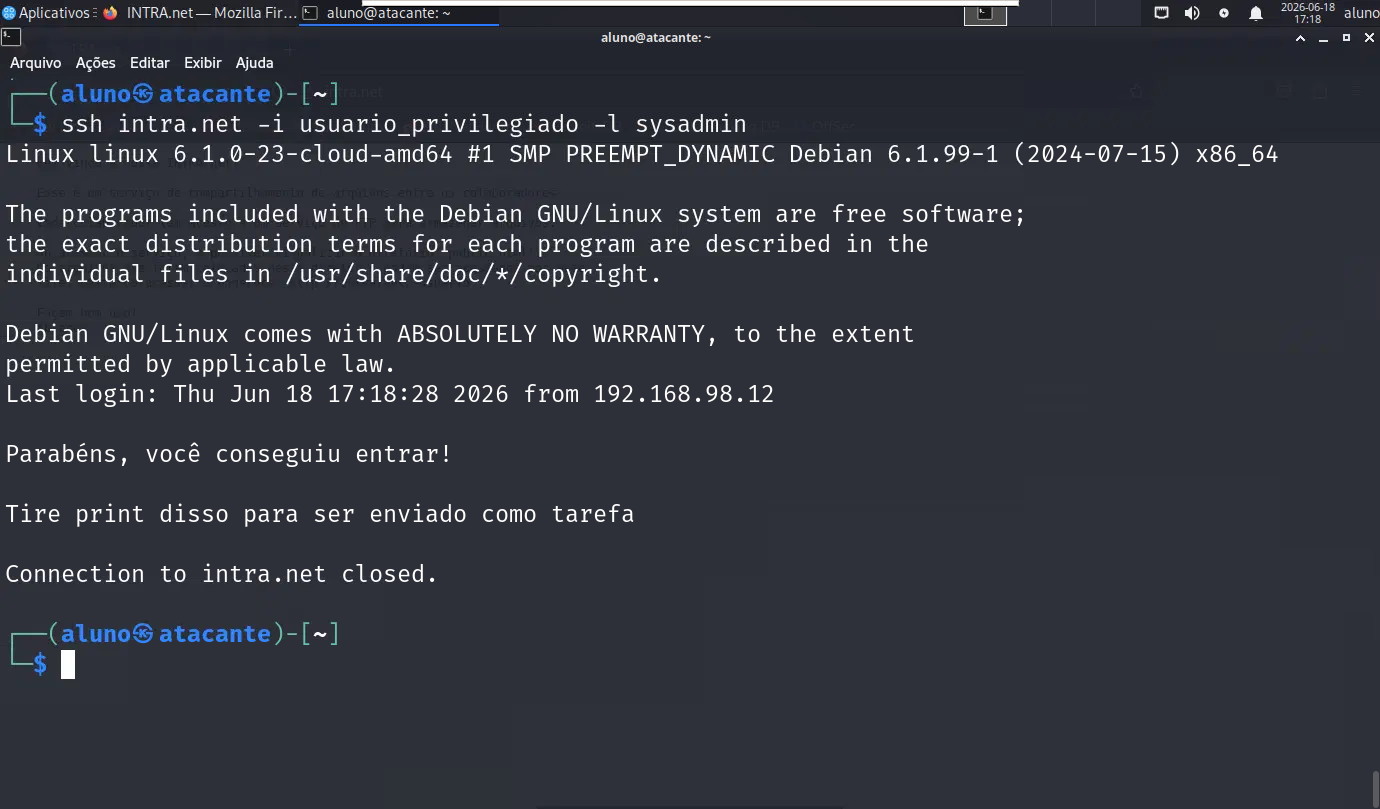
\includegraphics[width=0.95\textwidth]{./fig/login-ssh-privilegiado.png}
  \caption{Acesso SSH obtido utilizando chave privada exposta.}
  \label{fig:ssh-priv}
\end{figure}

\textbf{Impacto}

\begin{itemize}
  \item Comprometimento de conta privilegiada;
  \item Possibilidade de controle total do sistema;
  \item Acesso a informações sensíveis e recursos administrativos.
\end{itemize}

\textbf{Recomendação}

\begin{itemize}
  \item Armazenar chaves privadas de forma segura;
  \item Aplicar permissões restritivas aos arquivos sensíveis;
  \item Rotacionar imediatamente chaves expostas;
  \item Utilizar passphrase para proteção das chaves.
\end{itemize}

\subsection{Achado 04 -- Senha Previsível Baseada em Padrão Conhecido}

\textbf{Severidade: Média}

\paragraph{}
Foi identificado um padrão previsível na construção de senhas utilizado por um
usuário do ambiente.

\paragraph{}
A partir desse padrão foi criada uma expressão regular utilizada para gerar uma
wordlist direcionada. O conjunto reduzido de combinações permitiu identificar a
senha válida do usuário por meio de tentativa automatizada.

\textbf{Impacto}

\begin{itemize}
  \item Redução significativa do esforço necessário para ataques;
  \item Maior probabilidade de comprometimento de contas.
\end{itemize}

\textbf{Recomendação}

\begin{itemize}
  \item Utilizar senhas aleatórias;
  \item Evitar padrões previsíveis;
  \item Adotar gerenciadores de senha.
\end{itemize}

\subsection{Achado 05 -- Utilização de Hash MD5 para Armazenamento de Senhas}

\textbf{Severidade: Alta}

\paragraph{}
Foi identificado o uso do algoritmo MD5 para armazenamento de senhas.

\paragraph{}
As hashes obtidas foram submetidas ao processo de quebra utilizando a ferramenta
John the Ripper, resultando na recuperação das credenciais associadas.

\textbf{Impacto}

\begin{itemize}
  \item Comprometimento das credenciais armazenadas;
  \item Possibilidade de reutilização de senhas em outros sistemas;
  \item Aumento da superfície de ataque da organização.
\end{itemize}

\textbf{Recomendação}

\begin{itemize}
  \item Descontinuar o uso de MD5;
  \item Utilizar algoritmos modernos como Argon2, bcrypt ou scrypt;
  \item Implementar salting adequado nas senhas.
\end{itemize}
